\chapter{Game Engines}\label{ch:gameengines}
Eine \textit{Game Engine} ist ein komplexes Software-Framework, das für die Erstellung, Entwicklung und Bereitstellung interaktiver digitaler Anwendungen konzipiert ist, vor allem für Videospiele, aber auch für Simulationen, Architekturvisualisierungen und vieles mehr. Dabei ist das Hauptziel einer Game Engine, eine Abstraktion der allgemeinen Videospielfunktionen anzubieten, damit Code und Spielkomponente in verschiedenen Projekten wiederverwendet werden können. Die Funktionen einer modernen Game Engine können eine Rendering-Engine für 2D- oder 3D-Grafiken, Handhabung von Inputs, Physik-Engine, Animationen, Speichermanagement und Prozess-Threading sein. Bei vielen Game Engines heutzutage verwenden Entwickler höhere Programmiersprachen, wie Java, C++ und C\#, zum Entwickeln der Skripte für die Spiele. Außerdem werden immer mehr Plattformen angeboten, für die die Spiele entwickelt werden können, sei es für Desktop-Umgebungen, Mobilgeräte oder Konsolen.\cite{andrade2015game}

In diesem Kapitel werden drei Game Engines genauer betrachtet. Es wird das populäre Game Engine Unity, das von Epic Games veröffentlichte Unreal Engine und das neuere Godot Engine angeschaut. Alle Game Engines bieten eine Vielzahl an Möglichkeiten an, den Spielstand von einem Spieler abzuspeichern und zu laden.
%--------------------------------------------------------------------------


%--------------------------------------------------------------------------
\section{Unity}
\textit{Unity} ist eine leistungsstarke und vielseitige Echtzeit-3D-Entwicklungsplattform zum Entwickeln von Videospielen und Filmen. Sie wurde 2005 von Unity Technologies entwickelt und wurde durch die intuitive Benutzeroberfläche schnell zu der meist verwendeten Game Engine der Welt. Unity bietet für Spieleentwickler eine breite Auswahl an Systemen, für das Programmieren von 2D- und 3D-Spielen, Simulationen oder interaktiven Anwendungen. Sei es Mobilspiele, Spiele für jegliche Betriebssysteme, wie Windows, MacOS oder Linux, oder Spiele für Konsolen, mit allen ist es möglich, Unity zu verwenden. Programmiert wird bei Unity hauptsächlich mit der Programmiersprache C\#.\cite{unityUnityEngine}\cite{vsmid2017comparison}

In diesem Kapitel wird eine Vielzahl an Möglichkeiten angeschaut, welche Unity anbietet, um Speicher- und Ladesysteme für das Speichern des Spielstandes aufzustellen. Als erstes wird Unitys PlayerPrefs-Klasse angeschaut. Danach werden verschiedene Arten aufgezählt, Objekte von Unity in \ac{json} zu serialisieren und wann welche Strategie Sinn macht. Anschließend werden sich die .NET-Klassen BinaryFormatter, StreamWriter und StreamReader angeschaut. Beim BinaryFormatter werden die Probleme beim Serialisieren und Deserialisieren von Daten erläutert und es werden Alternativen vorgestellt. Zum Schluss wird das kostenpflichtige Paket Easy Save aus dem Asset Store angeschaut, welches einfach und effizient ein komplettes Speicher- und Ladesystem für Spiele implementieren kann.

\subsection{PlayerPrefs}
Bei Speicher- und Ladesystemen bietet Unity für Entwickler wenige eingebaute Funktionen. Einer der wenigen Funktionen, die Unity bereitstellt, sind die PlayerPrefs. Sie eine einfache Art, Daten zu speichern, aber ist dabei auch sehr limitiert. Die PlayerPrefs-Klasse besitzt wenige Funktionen, denn es werden nur die Datentypen string, float und integer unterstützt. Über einen Schlüssel lässt sich dann ein Schlüsselwert dieser Datentyppen festlegen oder es kann dieser erhalten werden. Die Werte der PlayerPrefs-Klasse werden mit der klasseninternen Save-Funktion gespeichert. Diese kann während der Laufzeit im Code aufgerufen werden und wird automatisch bei der Terminierung des Spieles aufgerufen.\cite{unityPlayerPrefsSave} Je nach Betriebssystem werden die PlayerPrefs in einem unterschiedlichen Datei-Format abgespeichert, die Daten werden aber nicht verschlüsselt.\cite{unityPlayerPrefs}

Allgemein wird davon abgeraten, Unitys PlayerPrefs System für das Speichern des Spielstandes zu verwenden. Zum einen wird für ein Spiel eine Speicherdatei erstellt. Wenn es aber in dem Spiel verschiedene Spielstände geben soll, gibt es bereits Probleme mit diesem Ansatz. Eine mögliche Lösung von diesem Problem wäre es, dass jeder Spielstand eine Identifikationsnummer bekommt, welche dann an jedem Schlüssel hinzugefügt wird. Die ganzen Identifikationsnummern müssen aber auch gespeichert werden, wo auch schon das nächste Problem mit PlayerPrefs auftritt. Es gibt wenige verfügbare Datentypen, die verwendet werden können. Wenn zum Beispiel eine Liste der Identifikationsnummern aller Spielstände gespeichert werden soll, kann dies nicht so einfach gemacht werden. Über den string-Datentyp lassen sich jedoch \ac{json}-Strings speichern, wodurch wieder mehr Datentypen, wie Listen und andere Gruppierungen von Daten, möglich sind. Und PlayerPrefs, was für Player Preferences steht, ist eigentlich auch genaufür die Arten von Daten gemacht. Es sollten Konfigurationen, wie die Auflösung oder die Lautstärke des Spieles, gespeichert werden. Da die Daten auch alle in einer Datei gespeichert werden, ist es auch nicht sonderlich effizient mit vielen Daten zu arbeiten. Effizienter wäre es die Daten auf verschiedene Dateien aufzuteilen, um schnellere Ladezeiten zu erreichen.
\cite{unityPersistentData}\cite{logrocketPlayerPrefs}\cite{gamedevbeginnerPlayerPrefs}

\subsection{JSON}
Die verbreiteste Art mit Unity Spielstände abzuspeichern ist mit \ac{json}. Ein Grund dafür ist, dass Unity ein Tool für das Serialisieren von C\# Objekten hat. Dieses Tool heißt \textit{JsonUtility}, welches über Data Binding die Daten verarbeitet. JsonUtility hat zwar einige Einschränkungen, ist dafür aber die schnellste Art, Objekte in \ac{json} zu serialisieren. Eine Einschränkung von JsonUtility ist, dass es einige Typen gibt, die nicht unterstützt werden, wie Dictionary<>, multidimensionale oder Jagged\footnote{Jagged Arrays sind Arrays, dessen Elemente Arrays aus verschiedener Größe sind.\cite{microsoftVerzweigteArrays}} Arrays. Diese lassen sich nicht mit JsonUtility serialisieren. In dem Beielcode \ref{lst:jsonUtilityExp} werden die drei Funktionen, die JsonUtility anbietet, demonstriert. Von der Zeile 1 bis 7 wird eine Spieler-Klasse definiert, welche dann in einer anderen Klasse, wie ab der Zeile 11 zu sehen ist, verwendet wird. Diese muss mit dem Attribut "Serializable" gekenntzeichnet werden, damit diese auch serialisierbar ist. Alle Variablen, die in dieser Klasse public oder mit "[SerializeField]" gekenntzeichnet werden, werden beim Serialisierungsprozess betrachtet. Als erstes werden drei Spieler-Objekte definiert, welche in den Zeilen 15 bis 18 zu \ac{json}-Strings serialisiert werden. In der Zeile 16 ist zu sehen, wie einer der \ac{json}-Strings aussieht. Der Spieler mit dem Namen "Bob" wird dann in den letzten zwei Zeilen zwei mal überschrieben. Einmal mit den Werten der Spielerin "Alice" und einmal mit den Werten des Spielers "Tom". 
\cite{unityJsonUtility}\cite{unitySerializationRules} 
\begin{listing}[htp]
    \begin{minted}{csharp} 
        [Serializable]
        public class Player
        {
            public int level;
            public float health;
            public string name;
        }

        ...
        
        Player bob = new Player() { level = 1, health = 75.2f, name = "Bob" };
        Player alice = new Player() { level = 3, health = 100.0f, name = "Alice" };
        Player tom = new Player() { level = 2, health = 1.0f, name = "Tom" };

        string bobJson = JsonUtility.ToJson(bob);
        //  {"level":1,"health":75.2,"name":"Bob"}
        string aliceJson = JsonUtility.ToJson(alice);
        string tomJson = JsonUtility.ToJson(tom);

        bob = JsonUtility.FromJson<Player>(aliceJson);
        JsonUtility.FromJsonOverwrite(tomJson, bob);
    \end{minted}
    \caption{JsonUtility Beispielcode}
    \label{lst:jsonUtilityExp}
\end{listing}

Eine pupuläre Alternative zu JsonUtility ist die \textit{Newtonsoft.JSON} Bibliothek, auch bekannt als \textit{Json.NET}. Sie wird sehr häufig bei C\# Projekten verwendet, da sie einfach zu verenden ist und das Umwandeln zwischen .NET-Objekten und \ac{json} in schnellen Laufzeiten bewältigen kann.\cite{newtonsoftJsonNETNewtonsoft} Der Vorteil gegenüber JsonUtility ist, dass alle nicht serialisierbaren Klassen von JsonUtility mit Json.NET serialisierbar sind. Es ist beispielsweise möglich ein Dictionary<> zu serialisieren\cite{newtonsoftSerializeDictionary}\cite{newtonsoftDeserializeDictionary} oder jegliche Arten von Arrays. Json.NET wird auch seit der Unity Version 2018.4\footnote{Die Unity Version 2018.4 wurde 2019 veröffentlicht.\cite{unityDownloadArchive}} als Paket unterstützt.\cite{NewtonsoftJsonUnitySupport} Beim Serialisieren von Objekten werden auch bei Json.NET alle Variablen, die public sind, serialisiert. Um beim Serialisieren weniger Daten entstehen zu lassen bietet Json.NET einige Funktionen an, wie zuum Beispiel das Attribut "[JsonIgnore]", mit dem sich Variablen beim Serialisierungsprozess ignorieren lassen, oder die NullValueHandling Einstellung, mit der eingestellt werden kann, ob null-Werte gespeichert werden sollen. Dadurch, dass Json.NET viele Einstellungen anbietet, bei denen der komplette Serialisierungsprozess anpassbar ist, lassen sich die Laufzeiten für Projekte stark optimieren.\cite{newtonsoftReducingSerialized}\cite{newtonsoftPerformanceTips}

Eine weitere .NET-Bibliothek, die durchaus beliebt ist, ist \textit{LitJSON}. Auch diese ermöglicht es, .NET-Objekte in \ac{json} und umgekehrt zu konvertieren.\cite{litjsonLitJSONDocumentation}. LitJSON bietet zwar viel weniger Funktionen als Json.NET an, aber es ist mithilfe des JsonReader und JsonWriter möglich, über die LitJSON Streaming API zu serialisieren und somit eine eigene Serialisierung der Klassen zu konstruieren.\cite{litjsonLitJSONReaders} Es gibt auch eine Bibliothek, wo LitJSON etwas bearbeitet wurde, damit die .NET-Bibliothek auch für Unity verwendet werden kann.\cite{githubGitHubMervillUnityLitJson}

Wenn für das Unity Projekt mit \ac{json} die Spielstände gespeichert werden sollen, stellt sich die Frage, welche Serialisierungs Klasse oder Bibliothek sich besser eignet. Wie in der Abbildung \ref{fig:unityJsonPerformance} zu sehen, ist JsonUtility die schnellste Art Objekte in \ac{json} umzuwandeln und umgekehrt. Die schnellen Laufzeiten von JsonUtility haben auch den Preis, dass die Klasse etwas eingeschränkt ist und einfach gehalten wurde. Sobald es komplexere Datenstrukturen gibt, ist das Arbeiten mit JsonUtility eine große Herausforderung. Da könnte sich der Entwickler dann doch für Json.NET oder LitJSON entscheiden, da diese mehr Datentypen unterstützten. Wenn es wichtig ist, dass das Programm schnell Serialisieren soll, dann ist LitJSON die adäquatere Wahl zum Arbeiten mit \ac{json}. Falls das Deserialisieren möglichst schnell laufen soll, ist Json.NET geeigneter.

\begin{figure}[htp]
    \centering
    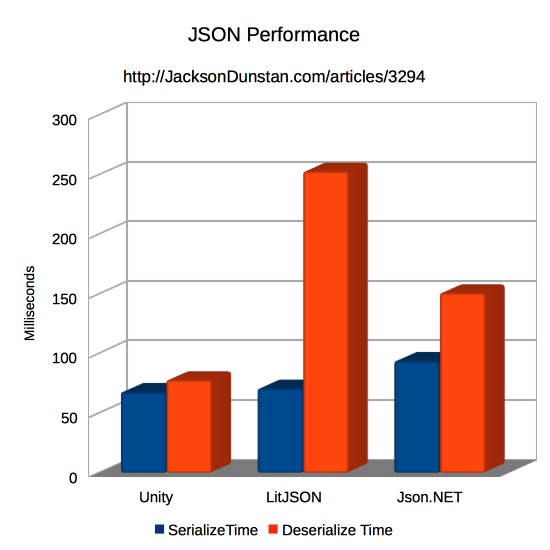
\includegraphics[width=0.6\textwidth]{images/UnityJsonPerformance.png}
    \caption{Laufzeiten der unterschiedlichen \ac{json} Serialisierer für Unity \cite{jacksondunstanJacksonDunstancomJSON}}
    \label{fig:unityJsonPerformance}
\end{figure}

\subsection{BinaryFormatter}\label{ssec:binaryFormatter}
Die .NET-Klasse \textit{BinaryFormatter} ist eine Möglichkeit eine binäre Serialisierung der Daten durchzuführen. Sie verwandelt .NET-Objekte in eine Liste von Bytes um und umgekehrt. In dem Beispielcode \ref{lst:binaryFormatterExp} ist zu sehen, wie der BinaryFormatter verwendet werden kann. Dabei werden die Player-Klasse und die Spieler aus dem Beispielcode \ref{lst:jsonUtilityExp} benutzt. In der Zeile 2 wird der Spieler namens "Bob" in der Datei "bobFile" in binärer Form abgespeichert. In der Zeile 3 wird das Objekt namens "tom" mit den Werten aus der "bobFile"-Datei neu gesetzt. Dabei werden die Daten aus "bobFile" wieder deserialisiert.\cite{microsoftBinaryFormatterClass} 

\begin{listing}[htp]
    \begin{minted}{csharp} 
        BinaryFormatter formatter = new BinaryFormatter();
        formatter.Serialize(bobFile,bob);
        tom = (Player) formatter.Deserialize(bobFile);
    \end{minted}
    \caption{Beispiel für das Serialisieren und Deserialisieren mit dem BinaryFormatter}
    \label{lst:binaryFormatterExp}
\end{listing}

Allgemein wird jedoch von dem Verwenden des BinaryFormatters abgeraten. Die Gefahr von Sicherheitsrisiken beim Deserialisieren ist zu groß. Ein Angreifer könnte den abgespeicherten Binärcode so verändern, dass dieser Code im Kontext des Zielprozesses ausführen wird. Je nach Anwendungstyp können solche Angriffe auch zu einem DoS-Angriff\footnote{Bei einem Denial of Service Angriff wird das Zielsystem mit etlichen Anfragen überflutet, was zu einer starken Verlangsamung, bis hin zu einem Zusammenbruch des Systems führen kann.\cite{bundDoSDDoSAttacken}} oder Veröffentlichung von Informationen führen.\cite{microsoftDeserializationRisks}

Eine sicherere Alternative zum BinaryFormatter sind die .NET-Klassen \textit{BinaryReader} und \textit{BinaryWriter}. Diese bieten Funktionalitäten an, zum Schreiben von primitiven Datentypen in Binärcode und zum Umwandeln von Binärcode in primitiven Datentypen. Mit dieser Methode ist es zwar aufwendiger die Daten zu speichern und zu laden, aber dafür sicherer als der BinaryFormatter.\cite{microsoftBinaryReaderClass}\cite{microsoftBinaryWriterClass}

\subsection{StreamWriter und StreamReader}
Eine weitere Alternative zu \ac{json} und dem binären Serialisieren der Daten mit Unity sind die .NET-Klassen StreamWriter und StreamReader. Mit dem StreamWriter lassen sich Zeilen in Dateien schreiben und mit dem StreamReader lassen sich diese dann lesen.\cite{microsoftStreamWriterKlasse}\cite{microsoftStreamReaderKlasse} Als Entwickler kann dann entschieden werden, ob Formate wie \ac{json}, Binärcode oder XML verwendet werden, oder ob zum Speichern der Daten ein eigenes Format konzipiert werden soll. Zum Beispiel können einfache Datenstrukturen, wie eine Liste von Identifikationsnummern, Zeile für Zeile in einer eigenen Datei gespeichert werden. Kompliziert wird es dann nur, wenn das Format zum Speichern der Daten geändert werden soll. Die alten Daten müssen dann alle in das neue Format übersetzt werden.

\subsection{Easy Save}
Für etwas Geld kann sich ein Entwickler das \textit{Easy Save} Paket vom Unity Asset Store anschauen. Dieses Tool bietet ein komplettes Speicher- und Ladesystem für Unity Projekte an, um eine einfache und effiziente Verwaltung der Daten zu ermöglichen.\cite{unityEasySave} In dem Beispielcode \ref{lst:easySaveExp} ist zu sehen, wie ein Wert in das Speichersystem mit aufgenommen werden kann, indem das Level des Spielers gespeichert und geladen wird. ES3 ist die Klasse von Easy Save und wie zu sehen ist, werden die Daten mit einem Schlüssel-Wert System gespeichert, ähnlich wie bei einem Dictionary.\cite{moodkieGettingStarted} Easy Save unterstützt viele Datentypen, wie Structs, Arrays, Wörterbücher, HashSets oder ganze Components\footnote{Die Basis-Klasse in Unity für alles was an den Spielobjekten (GameObject-Klasse) hinzugefügt wird.\cite{unityComponent}}.\cite{moodkieSupportedTypes} Falls ein Datentyp nicht von Easy Save unterstützt wird, kann man mit den ES3Types ganz einfach neue Datentypen zu dem System hinzufügen.\cite{moodkieChoosingWhat} Es ist auch möglich die gespeicherten Daten zu verschlüsseln oder zu komprimieren.\cite{moodkieGettingStarted} Vorausgesetzt die Daten sollen automatisch gespeichert, kann die "Auto Save" Funktion von Easy Save verwendet werden.\cite{moodkieAutoSave} Um eine bessere Leistung aus dem Speicher- und Ladesystem rauszuholen, kann mit Easy Save direkt eine Datei zum Speichern der Daten im Cache erstellt werden. Daten die dann dort gespeichert werden, können während der Laufzeit schneller geladen werden.\cite{moodkieImprovingPerformance}. Außerdem lassen sich Strings und Bytes direkt in den Speicherdateien schreiben und lesen.\cite{moodkieSavingLoading} 

\begin{listing}[htp]
    \begin{minted}{csharp} 
        int playerLevel = 1;
        ES3.Save("playerLevel", playerLevel);
        ... 
        if(ES3.KeyExists("playerLevel")) playerLevel = ES3.Load<int>("playerLevel")
    \end{minted}
    \caption{Beispiel für das Speichern und Laden mit Easy Save}
    \label{lst:easySaveExp}
\end{listing}

\subsection{Component-Save-System}

\url{https://github.com/AlexMeesters/Component-Save-System}

\subsection{Fazit}
Wann welches System bei Unity\dots
%--------------------------------------------------------------------------


%--------------------------------------------------------------------------
\section{Unreal Engine}
\textit{Unreal Engine} ist eine von Epic Games entwickelte Spiele-Engine, die von vielen größeren Entwicklungsteams verwendet wird. Unreal Engine ist aber auch bei einzelnen Entwicklern sehr beliebt, da es kostenlos und anfängerfreundlich ist. Bei realistischen Grafiken, Vegetation und Erstellung von Terrain für Videospiele liegt Unreal Engine auf Platz eins unter den Game Engines. Diese Enticklungsplattform ist vor allem für größere Projekte gemacht, obwohl es auch Unterstützung für iOS und Android gibt. Mithilfe der Blueprints lassen sich Spiele visueller erstellen. Blueprints sind Graphen, die aus Blöcken bestehen, die zusammen verbunden sind. Jeder Block hat dabei eine Funktion die ausgeführt wird. Beim Unreal Engine wird hauptsächlich mit der Programmiersprache C++ gearbeitet.\cite{vsmid2017comparison}

In diesem Abschnitt werden verschiedene Strategien betrachtet, die Unreal Engine anbietet, zum Speichern und Laden von Spielständen. Als erstes wird die Unreal Engine "SaveGame"-Klasse angeschaut, welche über C++-Code und Blueprints anbietet, ein vollständiges System zum Speichern und Laden von Daten aufzustellen. Anschließend wird betrachtet, welche Möglichkeit Unreal Engine anbietet, Daten in \ac{json} zu serialisieren und später diese zu deserialisieren. Zum Schluss wird ein Plugin für Unreal Engine 4 vorgestellt, mit dem in wenigen Schritten ein vollständiges Speicher- und Ladesystem aufgestellt werden kann. 

\subsection{SaveGame}
Seit Unreal Engine 4 wird die \textit{SaveGame} Klasse bereitgestellt. Sie bietet dem Entwickler ein fertiges Speicher- und Ladesystem für den Spielstand. Dies kann entweder in einem Blueprint oder mit C++ Code eingestellt werden. Die Daten werden dann alle im ".sav"-Format abgespeichert.
\cite{unrealengineSavingLoading}

Ein Beispiel für ein Blueprint zum Speichern der Spieldaten mit der SaveGame-Klasse ist in der Abbildung \ref{fig:unrealSaveGameBluePrintSave} zu sehen. Beim Erstellen dieses Blueprints muss als Elternklasse die SaveGame-Klasse ausgewählt werden, in diesem Beispiel heißt die Klasse "MySaveGame". In dieser Klasse können Variablen angelegt werden, die dann gespeichert und geladen werden sollen. Der Knoten "Create Save Game Object" in dem Blueprint erstellt eine neues Objekt der SaveGame-Klasse. In diesem Knoten muss dann "MySaveGame" als SaveGame-Klasse ausgewählt werden, damit mit den erstellten Variablen dieser Klasse gearbeitet werden kann. Mithilfe von "Set"-Knoten können die Werte der einzelnen Variablen in der eigenen SaveGame-Klasse gesetzt werden. Zum Speichern der Werte wird der "Save Game to Slot"-Knoten verwendet. Wenn das Speichern asynchron ablaufen soll, wird stattdessen der "Async Save Game to Slot"-Knoten verwendet, welcher von Epic Games empfohlen wird, wenn viele Daten gespeichert werden müssen. Dieser braucht als Eingabe ein SaveGame-Objekt, einen Slot-Namen und ein Benutzer-Index. Dabei wird der Slot-Name für den Namen der Speicherdatei und der Benutzer-Index als Benutzer-Identifikationsnummer verwendet. In dem Beispiel aus \ref{fig:unrealSaveGameBluePrintSave} werden für die Eingaben dieser die Standardwerte übergeben. Als Ausgabe-Pin gibt es einmal das SaveGame-Objekt der Eingabe und, ob das Speichern erfolgreich war.\cite{unrealengineSavingLoading}

\begin{figure}[htp]
    \centering
    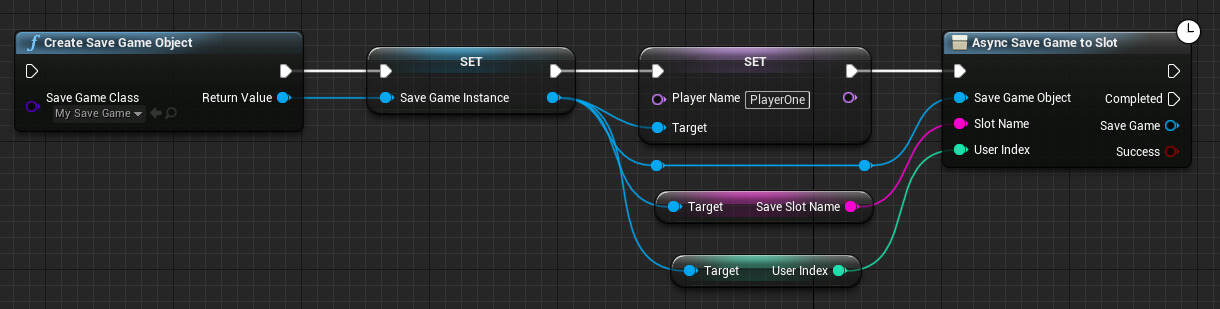
\includegraphics[width=1\textwidth]{images/SaveGameBP.png}
    \caption{Blueprint zum Speichern der Daten mit der SaveGame-Klasse\cite{unrealengineSavingLoading}}
    \label{fig:unrealSaveGameBluePrintSave}
\end{figure}

Wie das Laden der Spieldaten mit der SaveGame-Klasse funktioniert, ist in dem Blueprint der Abbildung \ref{fig:unrealSaveGameBluePrintLoad} zu sehen. Zu Beginn wird der "Load Game from Slot"-Knoten gebraucht, um die Daten zu laden. Falls viele Daten geladen werden, oder es während der Ladezeit ein Lade-Bildschirm geben soll, wird auch hier von Epic Games der "Async Load Game from Slot"-Knoten empfohlen, der das Gleiche wie der "Load Game from Slot"-Knoten macht, aber asynchron arbeitet. Als Eingabe braucht dieser Knoten den Slot-Namen und den Benutzer-Index. Der Ausgabewert muss dann zu der eigenen SaveGame-Klasse gecasted werden. Bei einem asynchronen Laden sollte zuerst mithilfe des "Is Valid"-Knotens überprüft werden, ob die Daten alle erfolgreich geladen wurden. Nach dem Cast zu der eigenen SaveGame-Klasse kann auf den Variablen dieser Klasse zugegriffen werden.\cite{unrealengineSavingLoading}

\begin{figure}[htp]
    \centering
    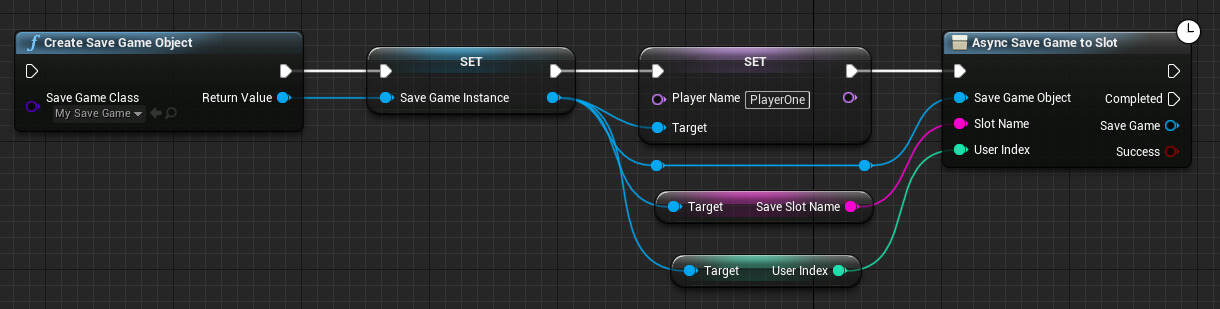
\includegraphics[width=1\textwidth]{images/SaveGameBP.png}
    \caption{Blueprint zum Laden der Daten mit der SaveGame-Klasse\cite{unrealengineSavingLoading}}
    \label{fig:unrealSaveGameBluePrintLoad}
\end{figure}

Falls dieses Speicher- und Ladesystem in C++-Code geschrieben werden soll, muss die Header-Datei "Kismet/GameplayStatics.h" zu der eigenen SaveGame-Klasse hinzugefügt werden und diese Klasse muss dann als Kind-Klasse von der USaveGame-Klasse deklariert werden. In der eigenen Klasse können dann die zu speichernden Variablen, der Slot-Name und der Benutzer-Index definiert werden. Mithilfe der Funktion SaveGameToSlot oder AsyncSaveGameToSlot und LoadGameFromSlot oder AsyncLoadGameFromSlot aus der Klasse UGameplayStatics können die Daten synchron oder asynchron gespeichert und geladen werden.\cite{unrealengineSavingLoading}

\subsection{JSON}
Auch bei Unreal Engine ist es möglich die Spieldaten im \ac{json}-Format abzuspeichern. Bei den Blueprints ist der Entwickler etwas eingeschränkt, da es erst seit Unreal Engine 5 Blueprints zum Arbeiten mit \ac{json} gibt, und die Anzahl der Funktionen noch gering ist. Es gibt Knoten für Blueprints, bei denen ein
C++-Struct zu einem \ac{json}-String umgeandelt wird oder Knoten, bei denen bestimmte Schlüsselwerte von \ac{json}-Objekten zurück gegeben werden. Außerdem gibt es Knoten, die \ac{json}-Objekte aus Dateien speichern und laden können.\cite{unrealengineJsonBlueprint}

Mehr Möglichkeiten gibt es beim direkten Arbeiten mit C++, um zu \ac{json} zu serialisieren. Dafür gibt es auch bei Unreal Engine eine \textit{JsonUtility}-Klasse. Zum Speichern der \ac{json}-Daten als C++-Objekt kann die FJsonObject-Klasse verwendet werden. Zum Serialisieren und Deserialisieren wird der FJsonSerializer benutzt. In dem Beispielcode \ref{lst:unrealFJsonSerializer} ist zu sehen, wie diese Klassen verwendet werden können. In den ersten vier Zeilen wird ein neues \ac{json}-Objekt erstellt, mit Schlüssel und Schlüsselwerten wie bei dem Code \ref{lst:jsonUtilityExp}. Danach wird in der Zeile 8 dieses \ac{json}-Objekt zu einem \ac{json}-String konvertiert und in dem Objekt "JsonString" gespeichert. In der Zeile 12 wird dieser String wieder deserialisiert und in ein \ac{json}-Objekt namens "JsonObject" gespeichert. Falls das Deserialisieren erfolgreich abläuft, ist die Kondition aus der Zeile 12 wahr und der Code in der Zeile 14 kann ausgeführt werden.\cite{unrealengineFJsonObject}\cite{unrealengineFJsonSerializer}\cite{wraiythUsingJson1}\cite{wraiythUsingJson2}

\begin{listing}[htp]
    \begin{minted}[breaklines,frame=single]{cpp}
        TSharedPtr BobJsonObject = MakeShareable(new FJsonObject);
        BobJsonObject->SetNumberField("level", 1);
        BobJsonObject->SetNumberField("health", 75.2f);
        BobJsonObject->SetStringField("name", "Bob");
        
        FString JsonString;
        TSharedRef<TJsonWriter<>> Writer = TJsonWriterFactory<>::Create(&JsonString);
        FJsonSerializer::Serialize(BobJsonObject.ToSharedRef(), Writer);   
        
        TSharedPtr JsonObject;
        TSharedRef<TJsonReader<>> Reader = TJsonReaderFactory<>::Create(JsonString);
        if(FJsonSerializer::Deserialize(Reader, JsonObject)) 
        {
           ...
        }
    \end{minted}
    \caption{Beispiel für das Serialisieren und Deserialisieren von Daten zu \ac{json}}
    \label{lst:unrealFJsonSerializer}
\end{listing}

\subsection{Save Extension}
Falls ein Entwickler ein fertiges Speicher- und Ladesystem sucht, welches er in sein Spiel integrieren möchte, dann ist \textit{Save Extension} geeignet. Dieses Plugin wurde für Unreal Engine 4 gemacht und bietet eine Vielzahl an Funktionen an, die sowohl in C++-Code oder als Blueprint implementiert werden können.\cite{unrealengineSaveExtension}

Die ersten Schritte zum Aufstellen des Speicher- und Ladesystems mit der Save Extension über ein Blueprint ist in der Abbildung \ref{fig:unrealSaveExtensionBlueprint} zu sehen. Die zwei Knoten "Save Slot to Id" und "Load Slot from Id" werden verwendet, um Daten aus einem bestimmten Slot zu speichern und zu laden. Jeder Slot kann eine bestimmte Spielwelt von einem Spieler sein und wird in einer eigenen Datei gespeichert.\cite{piperiftPiperiftSaveSlot} Um einen bestimmten Slot auszuwählen, gibt es die Eingabe "Slot Id", wo die Slot-Nummer eingegeben werden kann. Beim Speichern kann auch ausgewählt werden, ob der alte Spielstand eines Slots überschrieben werden soll, falls einer existiert. Zum Auslösen des Speicherns oder Ladens gibt es eine einige Möglichkeiten. In der Abbildung \ref{fig:unrealSaveExtensionBlueprint} zum Beispiel wird das Speichern des Spielstandes dadurch ausgelöst, dass die Tasten K gedrückt wurde. Zum Laden muss in diesem Beispiel die Taste L gedrückt werden. Alternativ unterstüzt das Save Extension Plugin auch ein Auto-Save und Auto-Load. Beim Auto-Save wird automatisch der aktuelle Slot gespeichert und beim Auto-Load wird immer der letzte aktive Slot geladen. Ein Slot wird als aktiv markiert, wenn er geladen wird.\cite{piperiftPiperiftSaveSlot}\cite{piperiftPiperiftSaveBlueprint} 

\begin{figure}[htp]
    \centering
    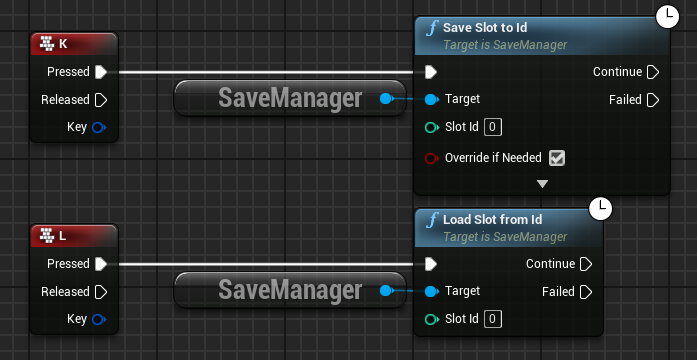
\includegraphics[width=0.8\textwidth]{images/SaveExtension_load_save_blueprint.png}
    \caption{Blueprint zum Laden der Daten mit dem Save Extension Plugin\cite{piperiftPiperiftSaveBlueprint}}
    \label{fig:unrealSaveExtensionBlueprint}
\end{figure}

Nach dieser Einrichtung werden noch keine Actor\footnote{Actors sind bei Unreal Engine alle Spielobjekte, die in der Spielwelt geladen werden.\cite{unrealengineActors}}-Klassen oder Components\footnote{Components werden an Actors angehangen und beeinflussen, wie diese sich verhalten.\cite{unrealengineActors}} gespeichert. Über das \textit{SavePreset} Blueprint lassen sich Actors und Component-Klassen zum Speicher- und Ladesystem hinzufügen. Um dann Variablen eines Actors oder Components abzuspeichern, muss für jede zu speichernde Variable die "SaveGame"-Eigenschaften angeklick werden. Komprimierung der Daten ist bei der Save Extension auch möglich. Dies kann bei dem SavePreset eingestellt werden.

Um zu vermeiden, dass zu viel Daten geladen werden, werden Slots in zwei Bereiche unterteilt und gespeichert. Es gibt einmal die Slot Info, die leichtgewichtete Daten über die Spielwelt speichert. Diese enthält zum Beispiel das Level des Spielers, seinen Spielername oder in welchem Bereich der Spielwelt sich der Spieler bei dem Spielstand befindet. Der Rest wird im "Slot Data"-Bereich gespeichert. Hier sind alle Informationen der serialisierten Actors und Components der Spielwelt eines Slots. Diese Unterteilung ist besonders praktisch, wenn wenige Slot-Informationen benötigt werden, aber diese nicht komplett geladen werden sollen. Falls zum Beispiel ein Menü erstellt wird, wo ausgewählt werden kann, mit welcher Spielwelt weitergespielt werden soll, kann hier bei jeder Spielwelt ein paar Informationen über diese beschrieben werden, ohne alle Slots komplett zu laden.\cite{piperiftPiperiftSaveSlot}

Eine weitere Funktion, die die Effizienz des Speicherns enorm verbessern kann, ist die Möglichkeit asynchron zu arbeiten. Bei dem Save Extension Plugin gibt es einmal die Multithreaded oder Frame-splitted Serialisierung, bei denen die zu serialisierenden Daten auf allen verfügbaren CPU-Threads oder auf mehreren Frames verteilt und dort einzeln serialisiert werden. Außerdem gibt es noch Multithreaded Dateien, die asynchron im Hintergrund der Anwendung komprimiert, gespeichert und geladen werden.\cite{piperiftPiperiftSaveMultithreaded}

Der Speicherprozess besteht aus den folgenden Schritten: Als Erstes wird der alte Spielstand gelöscht und es wird die Funktion OnSaveBegan aufgerufen, um weiterzugeben, dass der Speicherprozess begonnen hat. Dann werden der Thumbnail des aktuellen Spieles und die Spielstatistiken abgespeichert und anschließend wird die Spielwelt serialisiert. Zum Schluss wird die Funktion OnSaveFinished aufgerufen, um weiterzugeben, dass der Speicherprozess beendet wurde. In der Abbildung \ref{fig:piperiftSaveProcess} ist der vollständige Speicherprozess zu sehen. Gestrichelte Kanten bedeuten, dass hier mehrere Prozess parallel laufen können.\cite{piperiftSaveProcess}

\begin{figure}[htp]
    \centering
    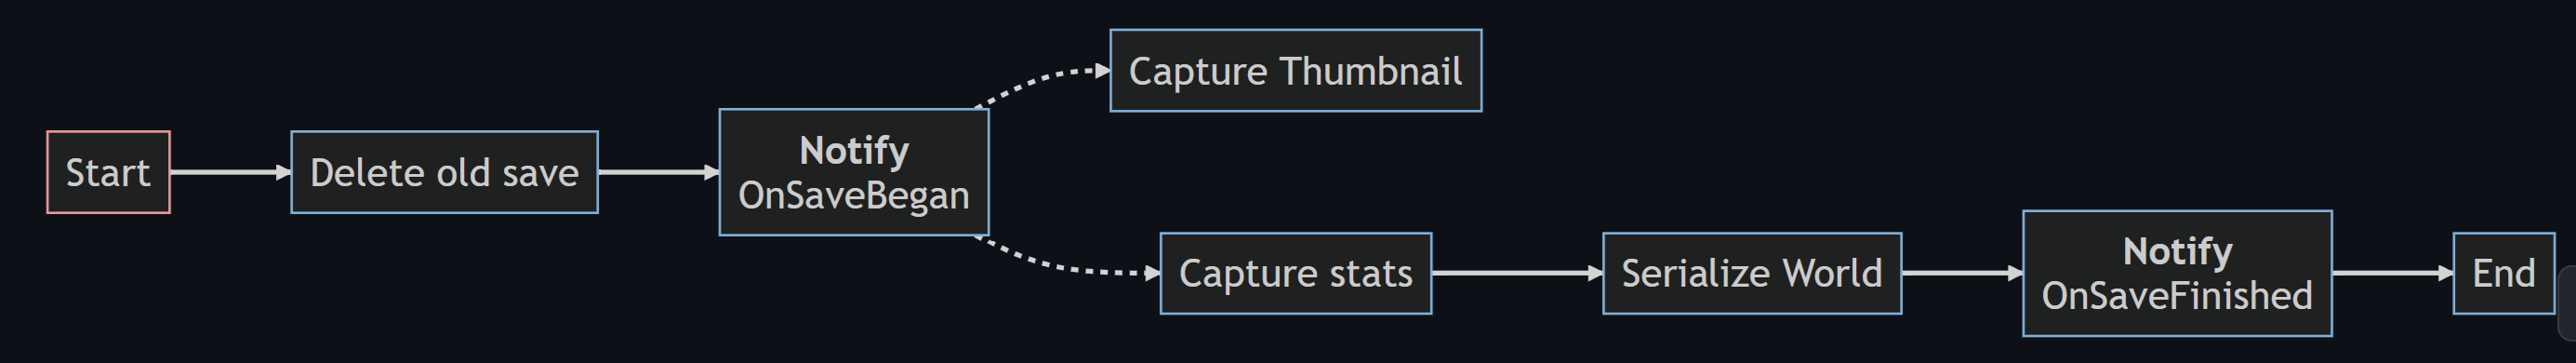
\includegraphics[width=1\textwidth]{images/piperift_save_process.png}
    \caption{Speicherprozess der Save Extension\cite{piperiftSaveProcess}}
    \label{fig:piperiftSaveProcess}
\end{figure}

Der Ladeprozess ist etwas komplexer. Als erstes wird die Funktion OnLoadBegan aufgerufen, um den Start des Ladeprozesses weiterzugeben. Danach werden alle Maps und Daten geladen und anschließen werden die Filter der einzelnen Level und generelle Filter vorbereitet, damit überprüft werden kann, welcher Actor in welchem Level geladen werden muss und wie dieser deserialisiert werden soll. Hiernach werden die einzelnen Levels vorbereitet und die Welt wird deserialisiert. Beim Vorbereiten der Levels werden gespeicherte Actors wiederhergestellen und nicht mehr existierende endgültig gelöscht. Bei dem Deserialisieren der Welt werden alle Level abgearbeitet und Actors und Components dieser deserialisiert. Zum Schluss wird die Funktion OnLoadFinished aufgerufen, um weiterzugeben, dass der Ladeprozess terminiert hat. In der Abbildung \ref{fig:piperiftLoadProcess} ist der vollständige Ladeprozess zu sehen.\cite{piperiftLoadProcess}

\begin{figure}[htp]
    \centering
    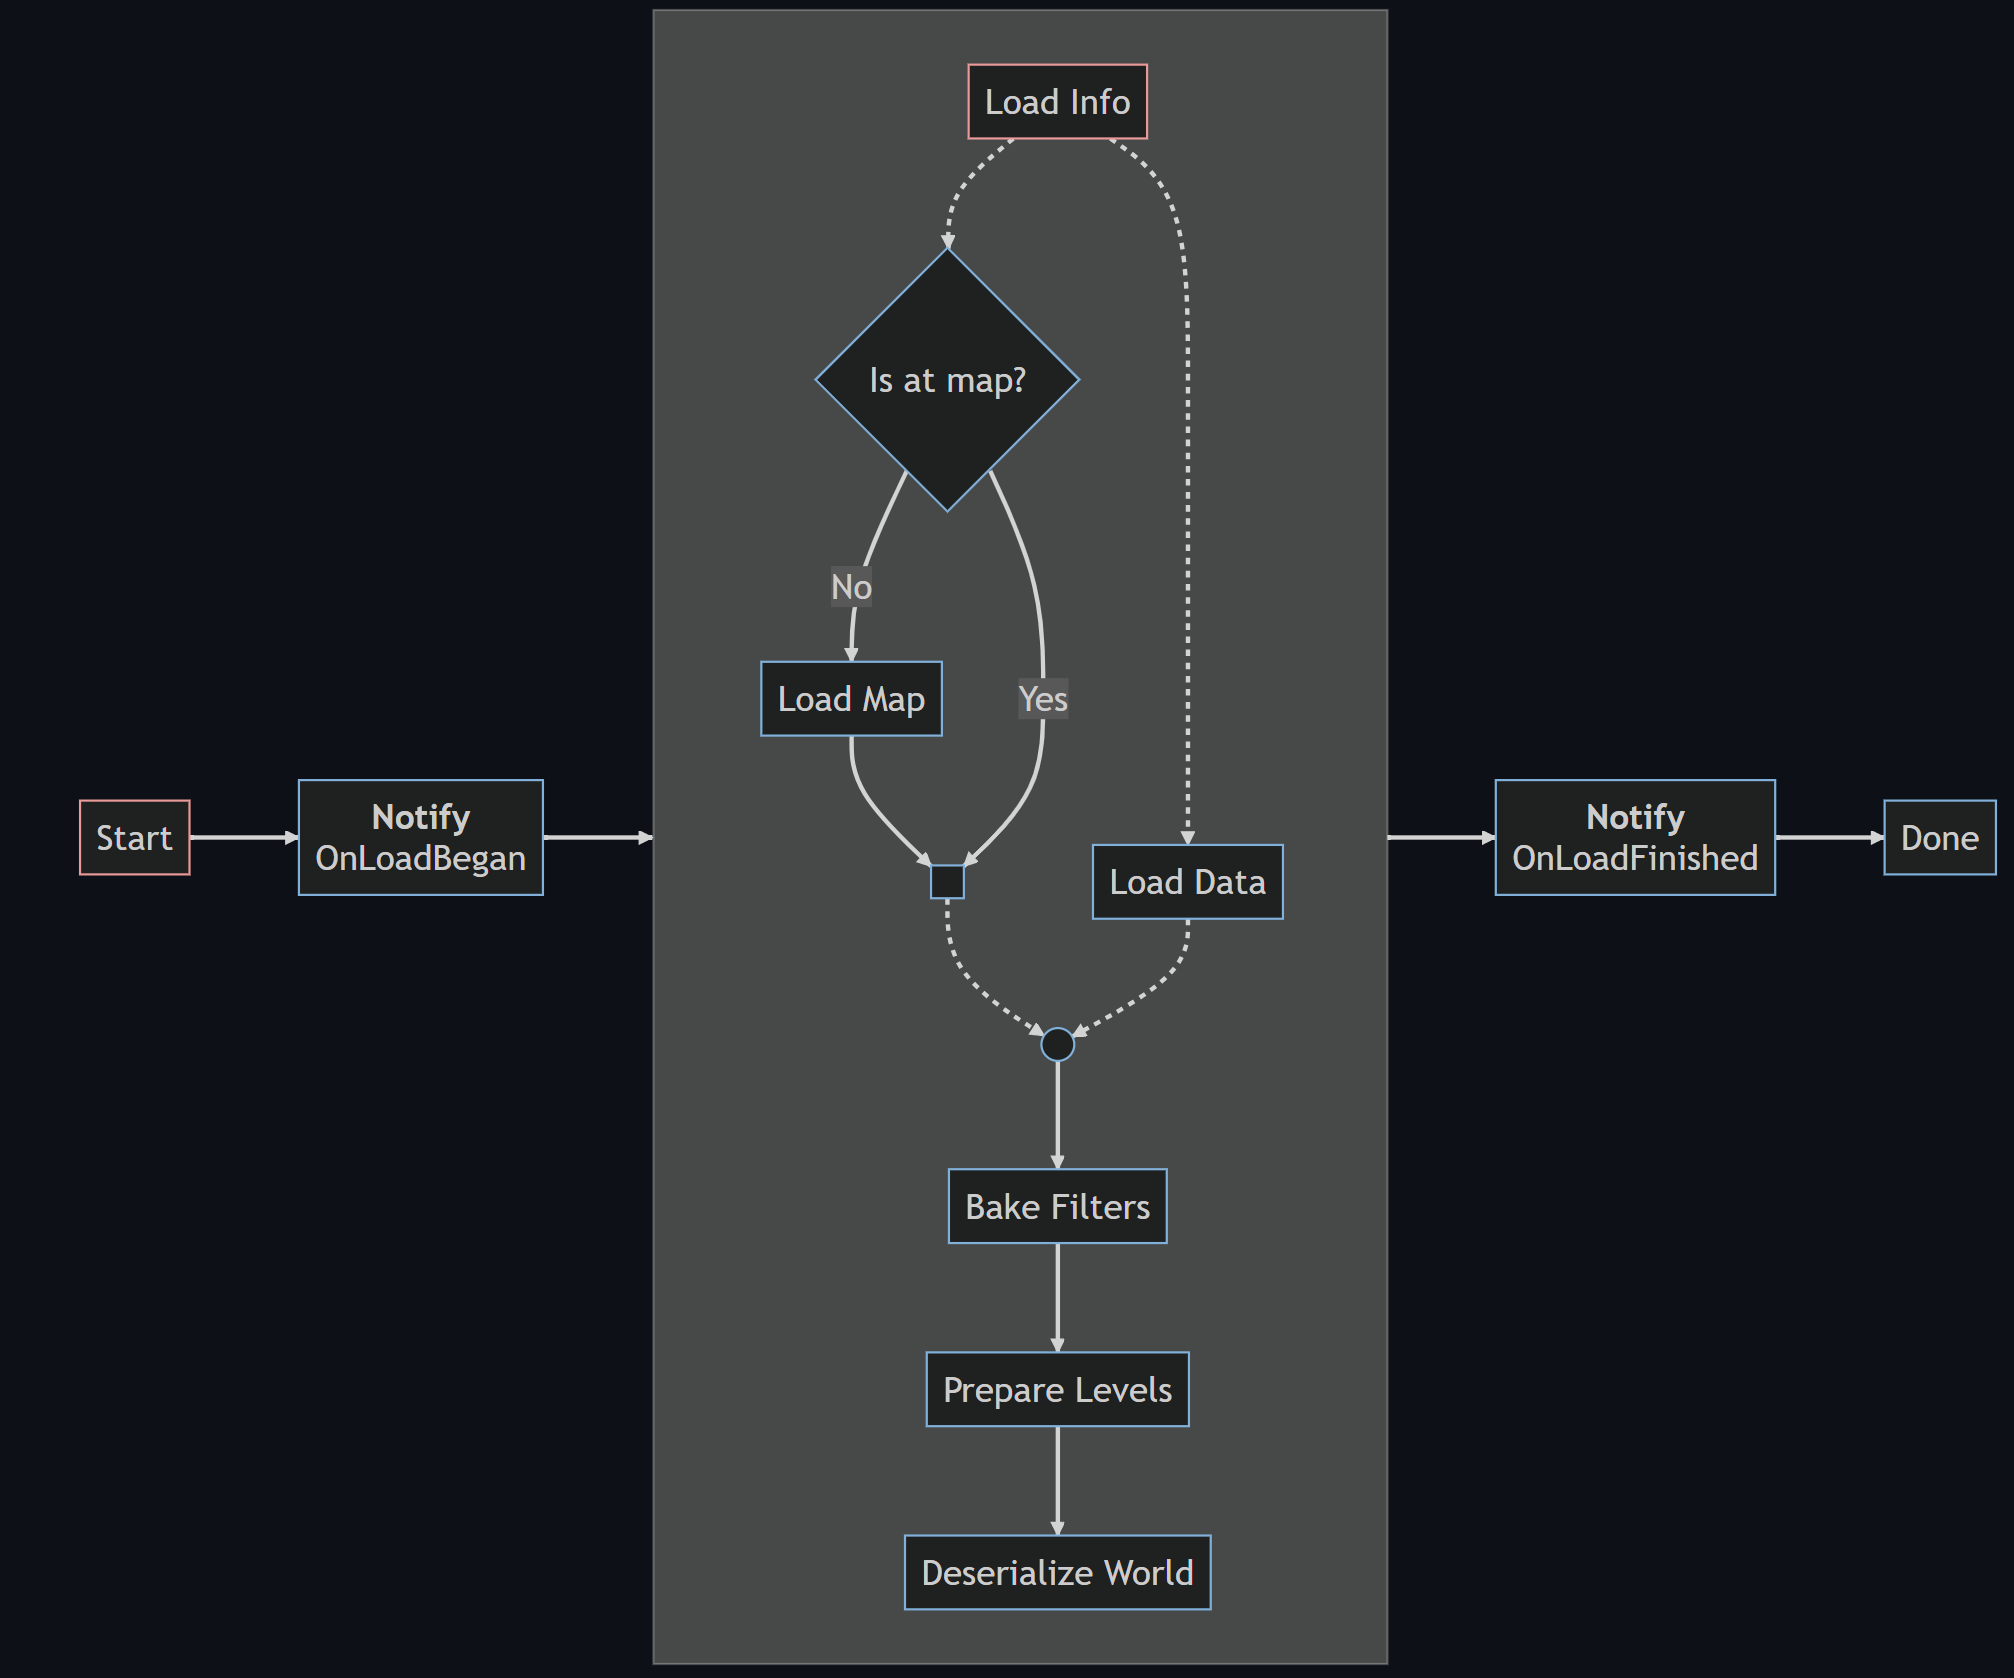
\includegraphics[width=0.8\textwidth]{images/piperift_load_process.png}
    \caption{Ladeprozess der Save Extension\cite{piperiftLoadProcess}}
    \label{fig:piperiftLoadProcess}
\end{figure}

\subsection{Fazit}
Wann welches System bei Unreal\dots
%--------------------------------------------------------------------------


%--------------------------------------------------------------------------
\section{Godot}
Godot Engine ist ein open-source und kostenfreies Game Engine, welches von einer Gemeinschaft von unabhängigen Entwicklern erstellt wurde. Es wurde 2014 veröffentlicht und wird hauptsächlich für kleinere Spiele verwendet, da es im Vergleich zu anderen Game Engines bei den Funktionen noch recht eingeschränkt ist. Im Vergleich zu Unity und Unreal Engine verwendet Godot keinen komponentenbasierten Ansatz, sondern hat verschiedene Klassen von Objekten, die Nodes genannt werden. Diese werden in einer Hierarchie in der Spiel-Szene angeordnet und jedem Node kann ein Skript angehangen werden, um das Verhalten dieser anzupassen. Statt bereits existierende Programmiersprachen zu verwenden, wurde für Godot eine eigene Programmiersprache entwickelt, namens GDScript, welche viele Ähnlichkeiten zu Python besitzt. Alternativ kann aber auch C\# und C++ zum Entwickeln von Spielen verwendet werden. Mit dem Godot Engine können 2D- und 3D-Spiele für Desktop-Plattformen, Mobilgeräte und das Web entwickelt werden.\cite{salmela2022game}

Zu Beginn von diesem Abschnitt werden zwei Möglichkeiten angeschaut, die von Godot Engine angeboten werden, um Spielobjekte zu serialisieren und deserialisieren. Einmal wird das Arbeiten mit \ac{json} betrachtet und danach die binäre Serialisierung. Zum Schluss wird noch ein Godot Plugin vorgestellt, welches ein fertiges Speicher- und Ladesystem für Entwickler anbietet. 

\subsection{JSON}
Da die Programmiersprache GDScript Dictionaries unterstützt, ist es sinnvoll mit \ac{json} arbeiten, da diese im GDScript bereits eine sehr \ac{json}-ähnliche Struktur besitzen. Um ein Speicher- und Ladesystem mit Godot Engine im \ac{json}-Format aufzustellen, sollten zu Beginn erst einmal alle Objekte, die gespeichert werden sollen, markiert werden. Jedes Objekt kann zu einer Gruppe hinzugefügt werden. Gruppen sind Ansammlungen von Objekten mit einem bestimmten Namen, wobei jedes Objekt auch mehreren Gruppen zugehören kann. Danach muss zu allen Objekten, die gespeichert werden sollen, eine Funktion hinzugefügt werden, die das Objekt zu einem \ac{json}-Objekt umwandelt. Wie so eine Funktion aussehen kann, ist in dem Code \ref{lst:godotJsonToJsonFunc} zu sehen. Alle wichtigen Variablen eines Objektes werden in ein Dictionary gepackt und danach mithilfe der "\ac{json}"-Hilfsklasse zu einem \ac{json}-String umgewandelt. Diese Klasse hat aber auch Einschränkungen, was alles in \ac{json} umgewandelt werden kann. Zum Beispiel können Vektoren, wie der "position"-Vektor eines Objektes, nicht direkt in \ac{json} umgewandelt werden. Deshalb muss die Position über eine x und y Variable gespeichert werden, statt direkt den "position"-Vektor zu speichern.\cite{godotengineSavingGames}

\begin{listing}[htp]
    \begin{minted}[breaklines,frame=single,tabsize=2]{python}
        func to_json():
          var object_data = {
            "filename" : get_scene_file_path(),
            "parent" : get_parent().get_path(),
            "x" : position.x, 
            "y" : position.y,
            "level": level,
            "health": health,
            "name": name
          }

          return \ac{json}.stringify(object_data)
    \end{minted}
    \caption{Beispiel für das Speichern mit \ac{json} in Godot\cite{godotengineSavingGames}}
    \label{lst:godotJsonToJsonFunc}
\end{listing}

Die "to\_json"-Funktion kann zum Speichern aller Objektzustände verwendet werden. In dem Code \ref{lst:godotJsonSave} ist zu sehen, wie eine Speicherfunktion aussehen könnte. Dabei wird als erstes eine Datei definiert, in der die Daten gespeichert werden sollen. Danach werden alle Objekte aus der "Save"-Gruppe geholt und über diese Menge wird iteriert. Wenn ein Objekt gespeichert werden soll, muss es zu dieser Gruppe hinzugefügt werden. Für jedes Objekt dieser Gruppe wird erst einmal geschaut, ob dieses Objekt aus einer Datei instanziiert wurde und ob in diesem Objekt die "to\_json"-Funktion enthalten ist. Bei jedem Node gibt es die Variable "scene\_file\_path", welche als String speichert, aus welcher Datei das Objekt instanziiert wurde. Alle Kind-Nodes dieses Objektes haben bei dieser Variable einen leeren String.\cite{godotengineNode} Diese Nodes sollen beim Speichern übersprungen werden. Bei den restlichen Objekten wird die "to\_json"-Funktion aufgerufen und der \ac{json}-String der zurückgegeben wird, wird in die Speicherdatei geschrieben.\cite{godotengineSavingGames}

\begin{listing}[htp]
    \begin{minted}[breaklines,frame=single]{python}
        func save_game():
          var save_game = FileAccess.open("user://savegame.save", FileAccess.WRITE)
          var save_nodes = get_tree().get_nodes_in_group("Save")
          for node in save_nodes:
            if node.scene_file_path.is_empty() || !node.has_method("to_json"): 
              continue 

            var json_string = node.call("to_json")
            save_game.store_line(json_string)
    \end{minted}
    \caption{Beispiel für das Speichern mit \ac{json} in Godot\cite{godotengineSavingGames}}
    \label{lst:godotJsonSave}
\end{listing}

Für das Laden der Daten müssen etwas mehr Schritte durchgeführt werden. In dem Code \ref{lst:godotJsonLoad} ist zu sehen, wie ein Spiel in Godot über eine "load\_game"-Funktion geladen werden kann, abhängig von den letzten zwei GDScripts. Zu Beginn sollte überprüft werden, dass die Speicherdatei existiert. Wenn das der Fall ist, kann der Prozess fortgesetzt werden. Als nächstes wird geschaut, ob schon Objekte der "Save"-Group existieren. Diese müssen gelöscht werden, weil sonst beim Laden Duplikate entstehen könnten. Danach kann begonnen werden die Speicherdatei Zeile für Zeile abzulesen. Da die Objekte immer als einzeilige \ac{json}-Strings gespeichert werden, stellt jede Zeile in der Speicherdatei ein Objekt da. Dieses \ac{json}-Objekt wird dann über der "parse"-Funktion der \ac{json}-Hilfsklasse deserialisiert. Falls das Deserialisieren erfolgreich war, werden die Daten des Objektes an die "load\_node"-Funktion weitergegeben. Diese instanziiert das Objekt und setzt die Werte der gespeicherten Variablen\cite{godotengineSavingGames}

\begin{listing}[htp]
    \begin{minted}[breaklines,frame=single]{python}
        func load_game():
          if not FileAccess.file_exists("user://savegame.save"):
            return

          var save_nodes = get_tree().get_nodes_in_group("Save")
          for i in save_nodes:
            i.queue_free()

          var save_game = FileAccess.open("user://savegame.save", FileAccess.READ)
          while save_game.get_position() < save_game.get_length():
            var json_string = save_game.get_line()
            var json = JSON.new()

            var parse_result = json.parse(json_string)
            if not parse_result == OK: continue

            load_node(json.get_data())

        func load_node(node_data):
          var new_object = load(node_data["filename"]).instantiate()
          get_node(node_data["parent"]).add_child(new_object)
          new_object.position = Vector2(node_data["x"], node_data["y"])

          for key in node_data.keys():
            if key == "filename" or key == "parent" or key == "x" or key == "y":
              continue
            new_object.set(i, node_data[i])
    \end{minted}
    \caption{Beispiel für das Laden mit \ac{json} in Godot\cite{godotengineSavingGames}}
    \label{lst:godotJsonLoad}
\end{listing} 

\subsection{Binary Serialization}
Auch binäre Serialisierung wird von Godot unterstützt. Bei diesem Prozess werden die verschiedenen Datentypen zu einem Array von Bytes umgewandelt. Von Godot Engine werden 30 verschiedene Datentypen bereitgestellt, die im binären Format gespeichert werden können. Beim serialisieren werden die Daten in Pakete verpackt. Ein Paket ist ein Datentyp mit seinem Wert. Die ersten vier Bytes eines Pakets beschreiben den Datentypen und zum setzen von Flags. Jeder Datentyp ist als Zahl definiert, welche in dem Header binär geschrieben wird. Zum Beispiel ist der Datentyp "int" mit der Zahl 2 definiert und über Flags kann gespeichert werden, ob es ein 32-Bit oder 64-Bit Integer ist. Ab dem fünften Byte beginnt der Inhalt des Pakets. Dieser varriiert von Datentyp zu Datentyp. Bei Strings zum Beispiel wird in den ersten vier Bytes des Inhalts definiert, wie lang die Zeichenkette ist, und erst nach diesen vier Bytes wird der String-Inhalt bestimmt. Bei solchen Datentypen ist die Größe des Paketinhalts variabel und nicht fest definiert.\cite{godotengineBinarySerialization}

Objekte können über Godots "var\_to\_bytes\_with\_objects"-Funktion binär serialisiert und mit der "bytes\_to\_var\_with\_objects"-Funktion wieder deserialisiert werden. Beim Deserialisieren muss jedoch aufgepasst werden, dass die Daten keinen Code beinhalten, der ausgeführt werden kann. Es sollten immer nur Daten von vertrauten Quellen deserialisert werden, sonst wird es zu Problem kommen, die bei dem BinaryFormatter Abschnitt \ref{ssec:binaryFormatter} genauer beschrieben wurden.\cite{godotengineGlobalScope}

Die binäre Serialisierung hat viele Vorteile gegenüber der \ac{json} Serialisierung. Zum einen sind die Dateigrößen deutlich kompakter bei binären Daten, im Vergleich zu den gespeicherten \ac{json}-Strings. Außerdem unterstützt Godot viel mehr Datentypen, die binär, aber nicht zu \ac{json} serialisiert werden können. Bei eigenen Klassen braucht es auch eigene Logiken, zum kodieren und dekodieren dieser, um diese zu \ac{json} zu serialisieren. Bei binärer Serialiserung wird weniger eigene Logik benötigt.\cite{godotengineSavingGames}

\subsection{Thoth}
Falls ein fertiges Speicher- und Ladesystem gesucht wird, welches in das Projekt integriert werden soll, dann ist das Plugin \textit{Thoth} eine Alternative zu den eingebauten Godot Engine Funktionen. Dieses System wurde so entwickelt, dass es für jede Art von Spiel verwendet werden kann und speichert den Spielzustand in einem Format, welches ähnlich zu \ac{json} ist, ab.\cite{stupidratstudioGodotSaveLoad}

Um das System aufzustellen, muss das "Savestate"-Node von diesem Plugin hinzugefügt werden. Diese Node ist immer mit einer Speicherdatei verbunden und kann den Spielzustand zu einem beliebigen Zeitpunkt speichern. Im GDScript-Code \ref{lst:godotThoth} ist zu sehen, wie das "Savestate"-Node verwendet werden kann. Als erstes wird in dem Array "serializable\_collections" definiert, welche Objekte serialisiert werden sollen. In dem Beispielcode werden alle Kinder-Nodes, von dem "SaveObjects"-Node serialisiert. Bei jedem Objekt kann außerdem mit dem "serializable"-Array eingestellt werden, welche Variable gespeichert wird. In dem Objekt, dem der Code \ref{lst:godotThothObject} angehangen wird, werden zum Beispiel nur die Variablen "level", "health" und "name" gespeichert. Die Variable "effects" wird beim Serialisieren übersprungen. Zum Speichern und Laden müssen die Funktionen "save\_game" und "load\_game" aus dem Code \ref{lst:godotThoth} aufgerufen werden. Bei der Speicherfunktion müssen als erstes die gespeicherten Daten geladen werden, da vielleicht noch Informationen der alten Spielstände gebraucht werden. Anschließend kann der aktuelle Spielzustand serialisiert und dann gespeichert werden. Bei der Ladefunktion wird als erstes der letzte Spielzustand geladen und danach deserialisert. 

\begin{listing}[htp]
    \begin{minted}[breaklines,frame=single]{python}
        extends Node2D

        const serializable_collections = [
          "SaveObjects"
        ]

        @onready var savestate = get_node("Savestate")

        func save_game():
          savestate.load_game_state()
          savestate.pack_game_state(self)  
          savestate.save_game_state()

        func load_game():
          savestate.load_game_state()
          savestate.unpack_game_state(self)
    \end{minted}
    \caption{Beispiel für das Speichern und laden mit Thoth}
    \label{lst:godotThoth}
\end{listing} 

\begin{listing}[htp]
    \begin{minted}[breaklines,frame=single]{python}
        extends Node2D

        var level
        var health
        var name
        var effects

        const serializable = [
            "level",
            "health",
            "name"
        ]

        ...
    \end{minted}
    \caption{Beispiel für die Einstellung, welche Variablen serialisiert werden sollen}
    \label{lst:godotThothObject}
\end{listing} 

\subsection{Fazit}
Wann welches System bei Godot\dots